%% Kortsett fra mattelab.no – laget automatisk av bygg.py. Rediger gjerne til eget bruk.
%% Kompiler med lualatex.
\documentclass[11pt,a4paper]{article}
\usepackage[norsk]{babel}
\usepackage[a4paper,margin=1.2cm,bottom=1.7cm]{geometry}
\usepackage{fontspec}
\usepackage{unicode-math}
\setmainfont{TeX Gyre Pagella}
\setsansfont{TeX Gyre Heros}[Scale=MatchLowercase]
\setmathfont{TeX Gyre Pagella Math}
\usepackage{xcolor}
\definecolor{blekk}{HTML}{16213A}
\definecolor{dempet}{HTML}{566077}
\definecolor{m1}{HTML}{2F4AB0}
\usepackage{tikz}
\usepackage{qrcode}
\usepackage{fancyhdr}
\usepackage[hidelinks]{hyperref}
\pdfvariable suppressoptionalinfo \numexpr 1+2+4+8+16+32+64+128+256+512\relax
\setlength{\parindent}{0pt}
\setlength{\parskip}{0pt}
\pagestyle{fancy}
\fancyhf{}
\renewcommand{\headrulewidth}{0pt}
\fancyfoot[L]{\sffamily\footnotesize\color{dempet}mattelab.no · Velg metode for andregradslikninger · kortsett K7}
\fancyfoot[R]{\sffamily\footnotesize\color{dempet}Side \thepage}
\begin{document}
\begin{minipage}[t]{0.8\linewidth}\vspace{0pt}
{\sffamily\small\color{dempet}Kortsett K7 · 1T · mattelab.no}\par\vspace{0.25em}
{\fontsize{20}{24}\selectfont\bfseries Velg metode for andregradslikninger}\par\vspace{0.5em}
Sorter likningene etter hvilken metode du ville brukt for å løse dem raskest. Ofte finnes det flere gode svar. Begrunn valget, og løs gjerne likningen etterpå.\par\vspace{0.4em}{\small\color{dempet}Klipp langs de stiplede linjene. Koden nede i hjørnet (K7-01, K7-02, …) viser hvilket sett kortet hører til. De grå kortene er overskrifter for boksene.}
\end{minipage}\hfill
\begin{minipage}[t]{0.15\linewidth}\vspace{0pt}\raggedleft
\qrcode[height=1.9cm]{https://mattelab.no/varierende/velg-metode.html}
\end{minipage}\par\vspace{0.8em}

\noindent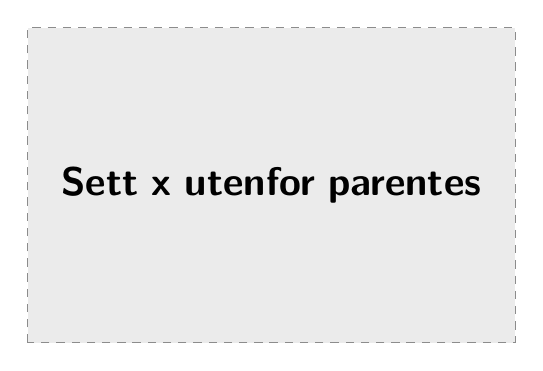
\begin{tikzpicture}
\useasboundingbox (0,0) rectangle (6.19,4.0);
\fill[black!8] (0,0) rectangle (6.19,4.0);
\node[text width=5.390000000000001cm, align=center, font=\sffamily\bfseries\Large] at (3.095,2.0) {Sett x utenfor parentes};
\draw[black!45, line width=0.4pt, dash pattern=on 3pt off 2.5pt] (0,0) rectangle (6.19,4.0);
\end{tikzpicture}%
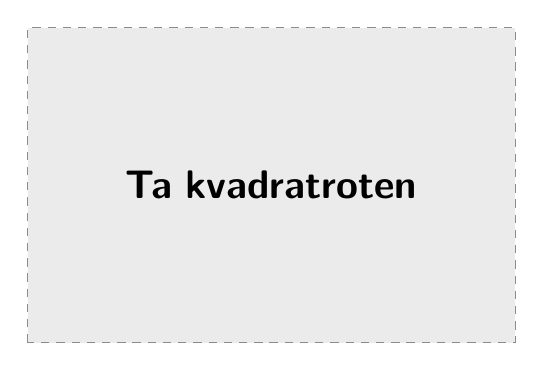
\begin{tikzpicture}
\useasboundingbox (0,0) rectangle (6.19,4.0);
\fill[black!8] (0,0) rectangle (6.19,4.0);
\node[text width=5.390000000000001cm, align=center, font=\sffamily\bfseries\Large] at (3.095,2.0) {Ta kvadratroten};
\draw[black!45, line width=0.4pt, dash pattern=on 3pt off 2.5pt] (0,0) rectangle (6.19,4.0);
\end{tikzpicture}%
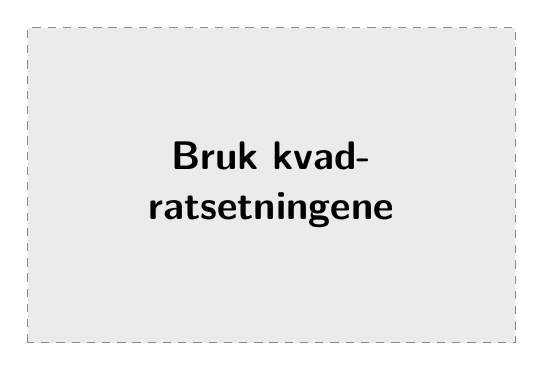
\begin{tikzpicture}
\useasboundingbox (0,0) rectangle (6.19,4.0);
\fill[black!8] (0,0) rectangle (6.19,4.0);
\node[text width=5.390000000000001cm, align=center, font=\sffamily\bfseries\Large] at (3.095,2.0) {Bruk kvadratsetningene};
\draw[black!45, line width=0.4pt, dash pattern=on 3pt off 2.5pt] (0,0) rectangle (6.19,4.0);
\end{tikzpicture}%
\par\nointerlineskip
\noindent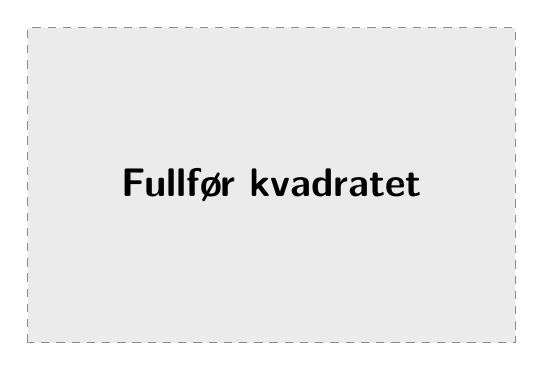
\begin{tikzpicture}
\useasboundingbox (0,0) rectangle (6.19,4.0);
\fill[black!8] (0,0) rectangle (6.19,4.0);
\node[text width=5.390000000000001cm, align=center, font=\sffamily\bfseries\Large] at (3.095,2.0) {Fullfør kvadratet};
\draw[black!45, line width=0.4pt, dash pattern=on 3pt off 2.5pt] (0,0) rectangle (6.19,4.0);
\end{tikzpicture}%
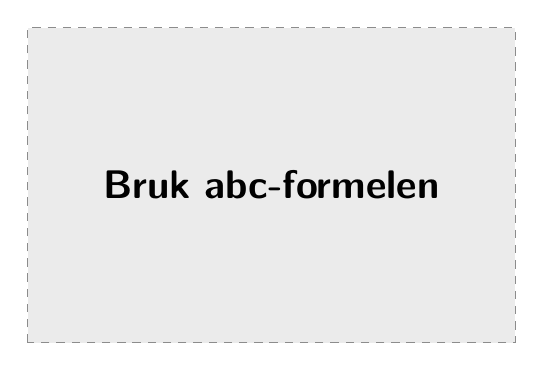
\begin{tikzpicture}
\useasboundingbox (0,0) rectangle (6.19,4.0);
\fill[black!8] (0,0) rectangle (6.19,4.0);
\node[text width=5.390000000000001cm, align=center, font=\sffamily\bfseries\Large] at (3.095,2.0) {Bruk abc-formelen};
\draw[black!45, line width=0.4pt, dash pattern=on 3pt off 2.5pt] (0,0) rectangle (6.19,4.0);
\end{tikzpicture}%
\begin{tikzpicture}
\useasboundingbox (0,0) rectangle (6.19,4.0);
\node[anchor=south east, font=\sffamily\scriptsize, text=black!40, inner sep=0pt] at (6.04,0.14) {Eget kort};
\draw[black!45, line width=0.4pt, dash pattern=on 3pt off 2.5pt] (0,0) rectangle (6.19,4.0);
\end{tikzpicture}%
\par\nointerlineskip
\noindent\begin{tikzpicture}
\useasboundingbox (0,0) rectangle (6.19,4.0);
\node[text width=5.29cm, align=center, font=\Large] at (3.095,2.08) {$x^2 - 5x = 0$};
\draw[black!45, line width=0.4pt, dash pattern=on 3pt off 2.5pt] (0,0) rectangle (6.19,4.0);
\node[anchor=south east, font=\sffamily\scriptsize, text=black!55, inner sep=0pt] at (6.04,0.14) {K7-01};
\end{tikzpicture}%
\begin{tikzpicture}
\useasboundingbox (0,0) rectangle (6.19,4.0);
\node[text width=5.29cm, align=center, font=\Large] at (3.095,2.08) {$x^2 + 2x = 8$};
\draw[black!45, line width=0.4pt, dash pattern=on 3pt off 2.5pt] (0,0) rectangle (6.19,4.0);
\node[anchor=south east, font=\sffamily\scriptsize, text=black!55, inner sep=0pt] at (6.04,0.14) {K7-02};
\end{tikzpicture}%
\begin{tikzpicture}
\useasboundingbox (0,0) rectangle (6.19,4.0);
\node[text width=5.29cm, align=center, font=\Large] at (3.095,2.08) {$x^2 + 4x - 5 = 0$};
\draw[black!45, line width=0.4pt, dash pattern=on 3pt off 2.5pt] (0,0) rectangle (6.19,4.0);
\node[anchor=south east, font=\sffamily\scriptsize, text=black!55, inner sep=0pt] at (6.04,0.14) {K7-03};
\end{tikzpicture}%
\par\nointerlineskip
\noindent\begin{tikzpicture}
\useasboundingbox (0,0) rectangle (6.19,4.0);
\node[text width=5.29cm, align=center, font=\Large] at (3.095,2.08) {$3x^2 + 5x - 2 = 0$};
\draw[black!45, line width=0.4pt, dash pattern=on 3pt off 2.5pt] (0,0) rectangle (6.19,4.0);
\node[anchor=south east, font=\sffamily\scriptsize, text=black!55, inner sep=0pt] at (6.04,0.14) {K7-04};
\end{tikzpicture}%
\begin{tikzpicture}
\useasboundingbox (0,0) rectangle (6.19,4.0);
\node[text width=5.29cm, align=center, font=\Large] at (3.095,2.08) {$x^2 - 16 = 0$};
\draw[black!45, line width=0.4pt, dash pattern=on 3pt off 2.5pt] (0,0) rectangle (6.19,4.0);
\node[anchor=south east, font=\sffamily\scriptsize, text=black!55, inner sep=0pt] at (6.04,0.14) {K7-05};
\end{tikzpicture}%
\begin{tikzpicture}
\useasboundingbox (0,0) rectangle (6.19,4.0);
\node[text width=5.29cm, align=center, font=\Large] at (3.095,2.08) {$(x - 2)^2 = 9$};
\draw[black!45, line width=0.4pt, dash pattern=on 3pt off 2.5pt] (0,0) rectangle (6.19,4.0);
\node[anchor=south east, font=\sffamily\scriptsize, text=black!55, inner sep=0pt] at (6.04,0.14) {K7-06};
\end{tikzpicture}%
\par\nointerlineskip
\noindent\begin{tikzpicture}
\useasboundingbox (0,0) rectangle (6.19,4.0);
\node[text width=5.29cm, align=center, font=\Large] at (3.095,2.08) {$2x^2 - 18 = 0$};
\draw[black!45, line width=0.4pt, dash pattern=on 3pt off 2.5pt] (0,0) rectangle (6.19,4.0);
\node[anchor=south east, font=\sffamily\scriptsize, text=black!55, inner sep=0pt] at (6.04,0.14) {K7-07};
\end{tikzpicture}%
\begin{tikzpicture}
\useasboundingbox (0,0) rectangle (6.19,4.0);
\node[text width=5.29cm, align=center, font=\Large] at (3.095,2.08) {$x^2 - 10x + 25 = 0$};
\draw[black!45, line width=0.4pt, dash pattern=on 3pt off 2.5pt] (0,0) rectangle (6.19,4.0);
\node[anchor=south east, font=\sffamily\scriptsize, text=black!55, inner sep=0pt] at (6.04,0.14) {K7-08};
\end{tikzpicture}%
\begin{tikzpicture}
\useasboundingbox (0,0) rectangle (6.19,4.0);
\node[text width=5.29cm, align=center, font=\Large] at (3.095,2.08) {$2x^2 - 3x - 4 = 0$};
\draw[black!45, line width=0.4pt, dash pattern=on 3pt off 2.5pt] (0,0) rectangle (6.19,4.0);
\node[anchor=south east, font=\sffamily\scriptsize, text=black!55, inner sep=0pt] at (6.04,0.14) {K7-09};
\end{tikzpicture}%
\par\nointerlineskip
\noindent\begin{tikzpicture}
\useasboundingbox (0,0) rectangle (6.19,4.0);
\node[text width=5.29cm, align=center, font=\Large] at (3.095,2.08) {$x^2 - 8x + 12 = 0$};
\draw[black!45, line width=0.4pt, dash pattern=on 3pt off 2.5pt] (0,0) rectangle (6.19,4.0);
\node[anchor=south east, font=\sffamily\scriptsize, text=black!55, inner sep=0pt] at (6.04,0.14) {K7-10};
\end{tikzpicture}%
\begin{tikzpicture}
\useasboundingbox (0,0) rectangle (6.19,4.0);
\node[text width=5.29cm, align=center, font=\Large] at (3.095,2.08) {$x^2 + 6x + 9 = 0$};
\draw[black!45, line width=0.4pt, dash pattern=on 3pt off 2.5pt] (0,0) rectangle (6.19,4.0);
\node[anchor=south east, font=\sffamily\scriptsize, text=black!55, inner sep=0pt] at (6.04,0.14) {K7-11};
\end{tikzpicture}%
\begin{tikzpicture}
\useasboundingbox (0,0) rectangle (6.19,4.0);
\node[text width=5.29cm, align=center, font=\Large] at (3.095,2.08) {$x^2 + x + 1 = 0$};
\draw[black!45, line width=0.4pt, dash pattern=on 3pt off 2.5pt] (0,0) rectangle (6.19,4.0);
\node[anchor=south east, font=\sffamily\scriptsize, text=black!55, inner sep=0pt] at (6.04,0.14) {K7-12};
\end{tikzpicture}%
\par\nointerlineskip
\noindent\begin{tikzpicture}
\useasboundingbox (0,0) rectangle (6.19,4.0);
\node[text width=5.29cm, align=center, font=\Large] at (3.095,2.08) {$3x^2 = 12x$};
\draw[black!45, line width=0.4pt, dash pattern=on 3pt off 2.5pt] (0,0) rectangle (6.19,4.0);
\node[anchor=south east, font=\sffamily\scriptsize, text=black!55, inner sep=0pt] at (6.04,0.14) {K7-13};
\end{tikzpicture}%
\begin{tikzpicture}
\useasboundingbox (0,0) rectangle (6.19,4.0);
\node[text width=5.29cm, align=center, font=\Large] at (3.095,2.08) {$x^2 = 49$};
\draw[black!45, line width=0.4pt, dash pattern=on 3pt off 2.5pt] (0,0) rectangle (6.19,4.0);
\node[anchor=south east, font=\sffamily\scriptsize, text=black!55, inner sep=0pt] at (6.04,0.14) {K7-14};
\end{tikzpicture}%
\begin{tikzpicture}
\useasboundingbox (0,0) rectangle (6.19,4.0);
\node[anchor=south east, font=\sffamily\scriptsize, text=black!40, inner sep=0pt] at (6.04,0.14) {Eget kort};
\draw[black!45, line width=0.4pt, dash pattern=on 3pt off 2.5pt] (0,0) rectangle (6.19,4.0);
\end{tikzpicture}%
\par\nointerlineskip
\noindent\begin{tikzpicture}
\useasboundingbox (0,0) rectangle (6.19,4.0);
\node[anchor=south east, font=\sffamily\scriptsize, text=black!40, inner sep=0pt] at (6.04,0.14) {Eget kort};
\draw[black!45, line width=0.4pt, dash pattern=on 3pt off 2.5pt] (0,0) rectangle (6.19,4.0);
\end{tikzpicture}%
\begin{tikzpicture}
\useasboundingbox (0,0) rectangle (6.19,4.0);
\node[anchor=south east, font=\sffamily\scriptsize, text=black!40, inner sep=0pt] at (6.04,0.14) {Eget kort};
\draw[black!45, line width=0.4pt, dash pattern=on 3pt off 2.5pt] (0,0) rectangle (6.19,4.0);
\end{tikzpicture}%
\begin{tikzpicture}
\useasboundingbox (0,0) rectangle (6.19,4.0);
\node[anchor=south east, font=\sffamily\scriptsize, text=black!40, inner sep=0pt] at (6.04,0.14) {Eget kort};
\draw[black!45, line width=0.4pt, dash pattern=on 3pt off 2.5pt] (0,0) rectangle (6.19,4.0);
\end{tikzpicture}%
\par\nointerlineskip
\end{document}
